\lab{Breadth-first Search}{Breadth-first Search}
\objective{
Shortest path problems are an important part of graph theory and network analysis.
Applications include finding the fastest way to drive between two points on a map, network routing, genealogy, automated circuit layout, and a variety of other important problems.
In this lab we represent graphs as adjacency dictionaries, implement a shortest path algorithm based on a breadth-first search, and use the NetworkX package to solve a shortest path problem on a large network of movies and actors.}

\section*{Adjacency Dictionaries} % ===========================================

Computers can represent mathematical graphs in various ways.
Graphs with very specific structures are often stored with specialized data structures, such as binary search trees.
More general graphs without structural constraints are usually represented with an \emph{adjacency matrix}, where each row and column of the matrix corresponds to a node in the graph, and the entries indicate connections between nodes.
Adjacency matrices are usually implemented in a sparse matrix format since only the entries corresponding to node connections are nonzero.

Another common graph data structure is an \emph{adjacency dictionary}, a dictionary with a key for each node in the graph.
The dictionary values are the set of nodes connected to the key node.
Adjacency dictionaries automatically gain the advantages of a sparse matrix format since they only store information on the actual node connections (the nonzero entries of the adjacency matrix).
% In Python, dictionaries are also much faster for lookup than matrices.

\begin{figure}[H] % simple graph, its adjacency matrix, and its adjacency dict.
\captionsetup[subfigure]{justification=centering}
\centering
\begin{subfigure}{.32\textwidth}
\centering
\begin{tikzpicture}[normalcircle/.style={draw,circle,minimum size=.75cm,fill=none,thick,node distance=1.5cm}]
    % Nodes
    \node[normalcircle] (A) [] {A};
    \node[normalcircle] (B) [above of=A] {B};
    \node[normalcircle] (C) [right of=B] {C};
    \node[normalcircle] (D) [below of=C] {D};
    % Edges
    \foreach \a/\b in {A/B,A/D,B/D,C/D} \draw[thick,-,>=stealth'] (\a) edge (\b);
\end{tikzpicture}
\end{subfigure}
%
\begin{subfigure}{.32\textwidth}
\centering
\begin{align*}
    \begin{blockarray}{ccccccc}
    & & \small\text{\textcolor{gray}{A}} & \small\text{\textcolor{gray}{B}} & \small\text{\textcolor{gray}{C}} & \small\text{\textcolor{gray}{D}} & \\
    \begin{block}{c[cccccc]}
    \small\text{\textcolor{gray}{A}} & & 0 & 1 & 0 & 1 & \topstrut\\
    \small\text{\textcolor{gray}{B}} & & 1 & 0 & 0 & 1 & \\
    \small\text{\textcolor{gray}{C}} & & 0 & 0 & 0 & 1 & \\
    \small\text{\textcolor{gray}{D}} & & 1 & 1 & 1 & 0 & \botstrut\\
    \end{block}\end{blockarray}
\end{align*}
\end{subfigure}
%
\begin{subfigure}{.32\textwidth}
\centering
\begin{align*}
\{\text{A}&:\ \{\text{B},\ \text{D}\},\\
  \text{B}&:\ \{\text{A},\ \text{D}\},\\
  \text{C}&:\ \{\text{D}\},\\
  \text{D}&:\ \{\text{A},\ \text{B},\ \text{D}\}\}
\end{align*}
\end{subfigure}
\caption{A simple unweighted graph (left), its adjacency matrix (middle), and its adjacency dictionary (right).
The graph is undirected, so the adjacency matrix is symmetric.
Note that the adjacency dictionary also encodes this behavior: since A and B are connected, B is in the set of values corresponding to the key A, and A is in the set of values corresponding to the key B.}
% There are eight $1$'s in the matrix, corresponding to $8$ total values in the dictionary.}
\label{fig:bfs-simple-graph}
\end{figure}

\subsection*{Hash-based Data Structures} % ------------------------------------

A Python \li{set} is an unordered data type with no repeated elements.
The set class is implemented as a \emph{hash table}, meaning it uses \emph{hash values}---integers that uniquely identify an object---to organize its elements.
Roughly speaking, in order to access, add, or remove an object \li{x} to a set, Python computes the hash value of \li{x}, and that value indicates where \li{x} is (or should be) in memory. % (usually with the built-in \li{hash()} function)
In other words, there is only one place in memory that \li{x} could be; if it isn't in that place, it isn't in the set.
This implementation results in $O(1)$ lookup, insertion, and removal operations, an enormous improvement over the $O(n)$ search time for lists and the $O(\log{n})$ search time for sorted structures like binary search trees.
It is also why set elements are unique.

\begin{table}[H]
\begin{tabular}{r|l}
    Method & Description\\
    \hline
    \li{add()} & Add an element to the set. This has no effect if the element is already present. \\
    \li{remove()} & Remove an element from the set, raising\\
    & a \li{KeyError} if it is not a member of the set.\\
    \li{discard()} & Remove an element from the set without raising \\
    & an exception if it is not a member of the set.\\
    \li{pop()} & Remove and return an arbitrary set element.\\
    \li{union()} & Return all elements that are in either set as a new set.\\
    \li{intersection()} & Return all elements that are in both sets as a new set.\\
    \li{update()} & Add all elements of another set in-place.
\end{tabular}
\caption{Basic methods of the \li{set} class.}
\end{table}

\begin{lstlisting}
# Initialize a set. Note that repeats are not added.
>>> animals = {"cow", "cat", "dog", "mouse", "cow"}
>>> print(animals)
<<{'cow', 'dog', 'mouse', 'cat'}>>

>>> animals.add("horse")     # Add an object to the set.
>>> "horse" in animals
<<True>>
>>> animals.remove("emu")    # Attempt to delete an object from the set,
<<KeyError: 'emu'>>              # resulting in an exception.
>>> animals.pop()            # Delete and return a random object from the set.
<<'mouse'>>
>>> print(animals)
<<{'cat', 'horse', 'dog', 'cow'}>>

# Add all of the elements of another set to this one.
>>> animals.update({"dog", "velociraptor"})
>>> print(animals)
<<{'velociraptor', 'cat', 'horse', 'dog', 'cow'}>>

# Intersect this set with another one.
>>> animals.intersection({"cat", "cow", "cheetah"})
<<{'cat', 'cow'}>>
\end{lstlisting}

Sets are extremely fast, but they do not support indexing because the elements are unordered.
A Python \li{dict}, on the other hand, is a hash-based data structure that stores key-value pairs: the keys of a dictionary act like a set (unique and unordered, with $O(1)$ lookup), but each key corresponds to another object, called its value.
The keys index the dictionary and allow $O(1)$ lookup of the values.

\begin{table}[H]
\begin{tabular}{r|l}
    Method & Description\\
    \hline
    \li{keys()} & Return a set-like iterator for the dictionary's keys.\\
    \li{values()} & Return a set-like iterator for the dictionary's values.\\
    \li{items()} & Return an iterator for the dictionary's key-value pairs.\\
    \li{pop()} & Remove a specified key and return the corresponding value,\\
    & raising a \li{KeyError} if the key is not a member of the dictionary.\\
    \li{update()} & Add or overwrite key-value pairs in-place with those from another dictionary.
\end{tabular}
\caption{Basic methods of the \li{dict} class.}
\end{table}

\begin{lstlisting}
# Initialize a dictionary.
>>> grades = {"business": "A", "math": "A+", "visual arts": "B"}
>>> grades["math"]
<<'A+'>>                            # The key "math" maps to the value "A+".

# Add a "science" key with corresponding value "A".
>>> grades["science"] = "A"

# Remove the "business" key.
>>> grades.pop("business")
<<'A'>>
>>> print(grades)
<<{'math': 'A+', 'visual arts': 'B', 'science': 'A'}>>

# Display the keys, values, and items.
>>> list(grades.keys()), list(grades.values())
<<(['math', 'visual arts', 'science'], ['A+', 'B', 'A'])>>
>>> for key, value in grades.items():
...   print(key, "=>", value)
...
<<math => A+
visual arts => B
science => A>>

# Add key-value pairs from another dictionary.
>>> grades.update({"cooking":"A+", "math": "C"})
>>> print(grades)
<<{'math': 'C', 'visual arts': 'B', 'science': 'A', 'cooking': 'A+'}>>
\end{lstlisting}

Dictionaries are ideal for storing values that need to be accessed often and for representing one-to-one or one-to-many relationships.
Thus, the \li{dict} class is a natural choice for implementing adjacency dictionaries.
For example, the following code defines the adjacency dictionary for the graph in Figure \ref{fig:bfs-simple-graph}.
Note that the dictionary values are sets.

\begin{lstlisting}
>>> adjacency = {'A': {'B', 'D'},
                 'B': {'A', 'D'},
                 'C': {'D'},
                 'D': {'A', 'B', 'C'}}

# The nodes of the graph are the dictionary keys.
>>> set(adjacency.keys())
<<{'B', 'D', 'A', 'C'}>>

# The values are the nodes that the key node is adjacent to.
>>> adjacency['A']
<<{'B', 'D'}>>                  # A is adjacent to B and D.
>>> 'C' in adjacency['B']
<<False>>                       # B and C are not adjacent.
>>> 'C' in adjacency['D']
<<True>>                        # C and D are adjacent.
\end{lstlisting}

\begin{warn} % hashable objects only
Elements of a \li{set} and keys of a \li{dict} must be \emph{hashable}.
Mutable objects---lists, sets and dictionaries---are not hashable, so they are not allowed as set elements or dictionary keys.
Thus, in order to represent a graph with an adjacency dictionary, each of the node labels should a string, a number, or some other hashable type.
\end{warn}


\begin{problem} % node, edge methods for Graph class (dictionary warm up).
\label{prob:bfs-graph-warmup}
Consider the following \li{Graph} class.
\begin{lstlisting}
class Graph:
    """A graph object, stored as an adjacency dictionary. Each node in the
    graph is a key in the dictionary. The value of each key is a set of
    the corresponding node's neighbors.

    Attributes:
        d (dict): the adjacency dictionary of the graph.
    """
    def __init__(self, adjacency={}):
        """Store the adjacency dictionary as a class attribute"""
        self.d = dict(adjacency)

    def __str__(self):
        """String representation: a view of the adjacency dictionary."""
        return str(self.d)
\end{lstlisting}
Add the following methods to this class.
\begin{enumerate}
\item \li{add_node()}: Add a node (with no initial edges) if it is not already present.
\\ (Hint: use \li{set()} to create an empty set.)
\item \li{add_edge()}: Add an edge between two nodes. Add the nodes to the graph if they are not already present.
\item \li{remove_node()}: Remove a node, including all edges adjacent to it.
This method should raise a \li{KeyError} if the node is not in the graph.
\item \li{remove_edge()}: Remove the edge between two nodes.
This method should raise a \li{KeyError} if either node is not in the graph, or if there is no edge between the nodes.
\end{enumerate}
\end{problem}

\section*{Breadth-first Search} % =============================================

Many common problems that arise in graph theory require finding the shortest path between two nodes in a graph.
For some highly structured graphs, such as binary search trees, this is a fairly straightforward problem (in the case of a tree, the shortest path is also the only path).
Finding a path between nodes in a graph of arbitrary structure, however, requires a careful and methodical approach.
The two most common graph search algorithms are \emph{depth-first search} (DFS) and \emph{breadth-first search} (BFS).
The breadth-first strategy is almost always better at finding shortest paths than the depth-first strategy,\footnote{See \url{https://xkcd.com/761/}.} though a DFS can be useful for path problems in certain graphs.

To traverse a graph with a BFS, choose a node to start at, called the \emph{source} node.
First, visit each of the source node's neighbors.
Next, visit each of the source node's neighbors' neighbors.
Then visit each of their neighbors, continuing the process until all nodes have been visited.
This strategy explores all of the nodes closest to the source node before incrementally moving ``deeper'' (further from the source node) into the tree.

The implementation of a BFS requires the following data structures to keep track of which nodes have already been visited and the order in which to visit nodes in future steps.
\begin{itemize}
    \item A list $V$: The nodes that have been \textbf{visited}, in visitation order.
    \item A \textbf{queue} $Q$: The nodes to be visited, in the order that they were discovered.
    Recall that a \emph{queue} is a limited-access list where data is inserted to one end, but removed from the other (first-in, first-out).
    \item A set $M$: The nodes that have been visited, or that are \textbf{marked} to be visited.
    This is the union of the nodes in $V$ and $Q$.
\end{itemize}
To begin the search, add the source node to $Q$ and $M$.
Then, until $Q$ is empty, repeat the following:
\begin{enumerate}
    \item Pop a node off of $Q$; call it the \emph{current} node.
    \item ``Visit'' the current node by appending it to $V$.
    \item Add the neighbors of the current node that are not in $M$ to $Q$ and $M$.
    \label{step:bfs-add-to-queue}
\end{enumerate}
The ``that are not in $M$'' clause of step \ref{step:bfs-add-to-queue} prevents nodes from being added to $Q$ more than once.
Note that step \ref{step:bfs-add-to-queue} could be replaced with ``Add the neighbors of the current node that are not in $V \cup Q$ to $Q$.''
However, lookup in $M$ (a set) is much faster than lookup in $V$ and $Q$ (arrays or linked lists), so including $M$ greatly speeds up the algorithm.

\begin{info}
The first-in, first-out (FIFO) structure of $Q$ enforces the ``breadth-first'' nature of the BFS: nodes that are marked first are visited first.
Using a a last-in, first-out (LIFO) stack for $Q$ changes the search to a DFS: the next node to visit is the one that was marked last.
\end{info}

\begin{figure}[H] % Example of a breadth-first search.
\captionsetup[subfigure]{justification=centering}
\centering
\begin{subfigure}{.6\textwidth}
    \centering
    \begin{tikzpicture}[normalcircle/.style={draw,circle,minimum size=.75cm,fill=none,thick,node distance=1.5cm}]
    % Nodes
    \node[normalcircle] (A) [fill=red!20] {A};
    \node[normalcircle] (B) [above of=A] {B};
    \node[normalcircle] (C) [right of=B] {C};
    \node[normalcircle] (D) [below of=C] {D};
    % Edges
    \foreach \a/\b in {A/B,A/D,B/D,C/D} \draw[thick,-,>=stealth'] (\a) edge (\b);
    \end{tikzpicture}
\end{subfigure}
%
\begin{subfigure}{.39\textwidth}
    \Large\begin{tabular}{r|l}
    $V$ & \textcolor{white}{A B C D} \\ \hline
    $Q$ & \textcolor{red}{A} \\ \hline
    $M$ & A \\
    \end{tabular}
\end{subfigure}
\\\vspace{20px}
\begin{subfigure}{.6\textwidth}
    \centering
    \begin{tikzpicture}[normalcircle/.style={draw,circle,minimum size=.75cm,fill=none,thick,node distance=1.5cm}]
    % Nodes
    \node[normalcircle] (A) [fill=blue!20] {A};
    \node[normalcircle] (B) [fill=red!20, above of=A] {B};
    \node[normalcircle] (C) [right of=B] {C};
    \node[normalcircle] (D) [fill=red!20, below of=C] {D};
    % Edges
    \foreach \a/\b in {B/D,C/D} \draw[thick,-,>=stealth'] (\a) edge (\b);
    \foreach \a/\b in {A/B,A/D} \draw[red!80,thick,->,>=stealth',line width=1.5pt] (\a) edge (\b);
    \end{tikzpicture}
\end{subfigure}
%
\begin{subfigure}{.39\textwidth}
    \Large\begin{tabular}{r|l}
    $V$ & \textcolor{blue}{A} \textcolor{white}{B C D} \\ \hline
    $Q$ & \textcolor{red}{B D} \\ \hline
    $M$ & A B D \\
    \end{tabular}
\end{subfigure}
\\\vspace{20px}
\begin{subfigure}{.6\textwidth}
    \centering
    \begin{tikzpicture}[normalcircle/.style={draw,circle,minimum size=.75cm,fill=none,thick,node distance=1.5cm}]
    % Nodes
    \node[normalcircle] (A) [fill=blue!20] {A};
    \node[normalcircle] (B) [fill=blue!20, above of=A] {B};
    \node[normalcircle] (C) [right of=B] {C};
    \node[normalcircle] (D) [fill=red!20, below of=C] {D};
    % Edges
    \foreach \a/\b in {A/B,A/D,B/D,C/D} \draw[thick,-,>=stealth'] (\a) edge (\b);
    \end{tikzpicture}
\end{subfigure}
%
\begin{subfigure}{.39\textwidth}
    \Large\begin{tabular}{r|l}
    $V$ & \textcolor{blue}{A B} \textcolor{white}{C D}\\ \hline
    $Q$ & \textcolor{red}{D} \\ \hline
    $M$ & A B D \\
    \end{tabular}
\end{subfigure}
\\\vspace{20px}
\begin{subfigure}{.6\textwidth}
    \centering
    \begin{tikzpicture}[normalcircle/.style={draw,circle,minimum size=.75cm,fill=none,thick,node distance=1.5cm}]
    % Nodes
    \node[normalcircle] (A) [fill=blue!20] {A};
    \node[normalcircle] (B) [fill=blue!20, above of=A] {B};
    \node[normalcircle] (C) [fill=red!20, right of=B] {C};
    \node[normalcircle] (D) [fill=blue!20, below of=C] {D};
    % Edges
    \foreach \a/\b in {A/B,A/D,B/D} \draw[thick,-,>=stealth'] (\a) edge (\b);
    \draw[red!80,thick,->,>=stealth',line width=1.5pt] (D) edge (C);
    \end{tikzpicture}
\end{subfigure}
%
\begin{subfigure}{.39\textwidth}
    \Large\begin{tabular}{r|l}
    $V$ & \textcolor{blue}{A B D} \\ \hline
    $Q$ & \textcolor{red}{C} \\ \hline
    $M$ & A B D C \\
    \end{tabular}
\end{subfigure}
\caption{To start a BFS from node A to node C, put A in the visit queue $Q$ and mark it by adding it to the set $M$.
Pop A off the queue and ``visit'' it by adding A to the visited list $V$ and the neighboring nodes B and D to $Q$.
Then visit B, but do not add anything to $Q$ because all of the neighbors of B are already marked.
Finally, visit D, at which point the target node C is located because it is adjacent to D.
}
\label{fig:bfs-example}
\end{figure}

\begin{problem} % BFS graph traversal.
\label{prob:bfs-traversal}
Write a method for the \li{Graph} class that accepts a source node.
Traverse the graph with a breadth-first search until all nodes have been visited.
Return the list of nodes in the order that they were visited.
If the source node is not in the graph, raise a \li{KeyError}.
\\(Hint: for $Q$, use a \li{deque} from the \li{collections} module, and make sure that nodes are added to one end but popped off of the other.)
\end{problem}

\subsection*{Shortest Paths via BFS} % ----------------------------------------

Consider the problem of locating a path between two nodes with a BFS.
The nodes that are directly connected to the source node are all visited before any other nodes; more generally, the nodes that are $n$ nodes away from the source node are all visited before nodes that are $n+1$ or more nodes from the source point.
Therefore, the search path taken to discover to the target with a BFS must be the shortest path from the source node to the target node.

Examine again the graph in Figures \ref{fig:bfs-simple-graph} and \ref{fig:bfs-example}.
The shortest path from A to C starts at A, goes to D, and ends at C.
During a BFS originating at A, D is placed on the visit queue because it is one of A's neighbors, and C is placed on the queue because it is one of D's neighbors.
Given that A was the node that visited D, and that D was the node that visited C, the shortest path from A to C can be constructed by stepping backward along the search path.

To implement this idea, initialize a dictionary before starting the BFS.
When a node is marked and added to the visit queue, add a key-value pair mapping the \textbf{visited} node to the \textbf{visiting} node (for example, B $\mapsto$ A means B was marked while visiting A).
When the target node is found, step through the dictionary until arriving at the source node, recording each step.

\begin{figure}[H] % Example of a breadth-first search.
\centering
\begin{tikzpicture}[normalcircle/.style={draw,circle,minimum size=.75cm,fill=none,thick,node distance=1.5cm}]
% Nodes
\node[normalcircle] (A) [fill=blue!20] {A};
\node[normalcircle] (B) [fill=blue!20, above of=A] {B};
\node[normalcircle] (C) [fill=blue!20, right of=B] {C};
\node[normalcircle] (D) [fill=blue!20, below of=C] {D};
% Edges
\draw[thick,-,>=stealth'] (B) edge (D);
\foreach \a/\b in {C/D,D/A,B/A} \draw[green!80,thick,->,>=stealth',line width=1.5pt] (\a) edge (\b);
\end{tikzpicture}
\caption{In the BFS from Figure \ref{fig:bfs-example}, nodes B and D were marked while visiting node A, and node C was marked while visiting node D (this is same as reversing the red arrows in Figure \ref{fig:bfs-example}).
Thus the ``visit path'' from C to A is $\text{C}\rightarrow\text{D}\rightarrow\text{A}$, so the shortest path from A to C is $[$A, D, C$]$.}
\label{fig:bfs-shortest-path}
\end{figure}

\begin{problem}
Add a method to the \li{Graph} class that accepts source and target nodes.
Begin a BFS at the source node and proceed until the target is found.
Return a list containing the node values in the shortest path from the source to the target (including the endpoints).
If either of the input nodes are not in the graph, raise a \li{KeyError}.
\label{prob:bfs-short-path1}
\end{problem}

\section*{Shortest Paths via NetworkX} % ======================================

\emph{NetworkX} is a Python package for creating, manipulating, and exploring graphs.
Its \li{Graph} object represents a graph with an adjacency dictionary, similar to the class from Problems \ref{prob:bfs-graph-warmup}--\ref{prob:bfs-short-path1}, and has many methods for interpreting information about the graph and its structure.
As before, the nodes must be hashable (a number, string, or another immutable object).

\begin{table}[H]
\centering
\begin{tabular}{r|l}
    Method & Description\\
    \hline
    \li{add_node()} & Add a single node to the graph.\\
    \li{add_nodes_from()} & Add a list of nodes to the graph.\\
    \li{add_edge()} & Add an edge between two nodes.\\
    \li{add_edges_from()} & Add a list of edges to the graph.
\end{tabular}
\caption{Methods of the \li{nx.Graph} class for adding nodes and edges.}
\end{table}

\begin{lstlisting}
>>> import networkx as nx

# Initialize a NetworkX graph from an adjacency dictionary.
>>> G = nx.Graph({'A': {'B', 'D'},
                  'B': {'A', 'D'},
                  'C': {'D'},
                  'D': {'A', 'B', 'C'}})

>>> print(G.nodes())            # Print the nodes.
<<['A', 'B', 'C', 'D']>>
>>> print(G.edges())            # Print the edges as tuples.
<<[('A', 'D'), ('A', 'B'), ('B', 'D'), ('C', 'D')]>>

>>> G.add_node('E')             # Add a new node.
>>> G.add_edge('A', 'F')        # Add an edge, which also adds a new node 'F'.
>>> G.add_edges_from([('A', 'C'), ('F', 'G')])  # Add several edges at once.

>>> set(G['A'])                 # Get the set of nodes neighboring node 'A'.
<<{'B', 'C', 'D', 'F'}>>
\end{lstlisting}

\subsection*{The Kevin Bacon Problem} % ---------------------------------------

The vintage parlor game \href{http://oracleofbacon.org/help.php}{\emph{Six Degrees of Kevin Bacon}} is played by naming an actor, then trying to find the shortest chain of actors that have worked with each other leading to Kevin Bacon.
For example, Samuel L. Jackson was in the film \emph{Pulp Fiction (1994)} with Frank Whaley, who was in \emph{JFK (1991)} with Kevin Bacon.
In other words, the goal of the game is to solve a shortest path problem on a graph that connects actors to the movies that they have been in.

\begin{problem} % MovieGraph.__init__()
The file \texttt{movie\_data.txt} contains IMDb data for about 137,000 movies.
Each line of the file represents one movie: the title is listed first, then the cast members, with entries separated by a \texttt{/} character.
For example, the line for \emph{The Dark Knight (2008)} starts with
\begin{center}
\texttt{The Dark Knight (2008)/Christian Bale/Heath Ledger/Aaron Eckhart/...}
\end{center}
Any \li{/} characters in movie titles have been replaced with the vertical pipe character \texttt{|} (for example, \texttt{Frost|Nixon (2008)}).

Write a class whose constructor accepts the name of a file to read.
Initialize a set for movie titles, a set for actor names, and an empty NetworkX \li{Graph}, and store them as attributes.
Read the file line by line, adding the title to the set of movies and the cast members to the set of actors.
Add an edge to the graph between the movie and each cast member.
\\(Hint: Use the \li{split()} method for strings to parse each line.)

It should take no more than 20 seconds to construct the entire graph.
Check that there are 137,018 movies and 930,717 actors.
Compare parts of your graph to Figure \ref{fig:bfs-network-subset}.
\label{prob:bfs-movie-network-init}
\end{problem}

\begin{figure}[H]
\centering
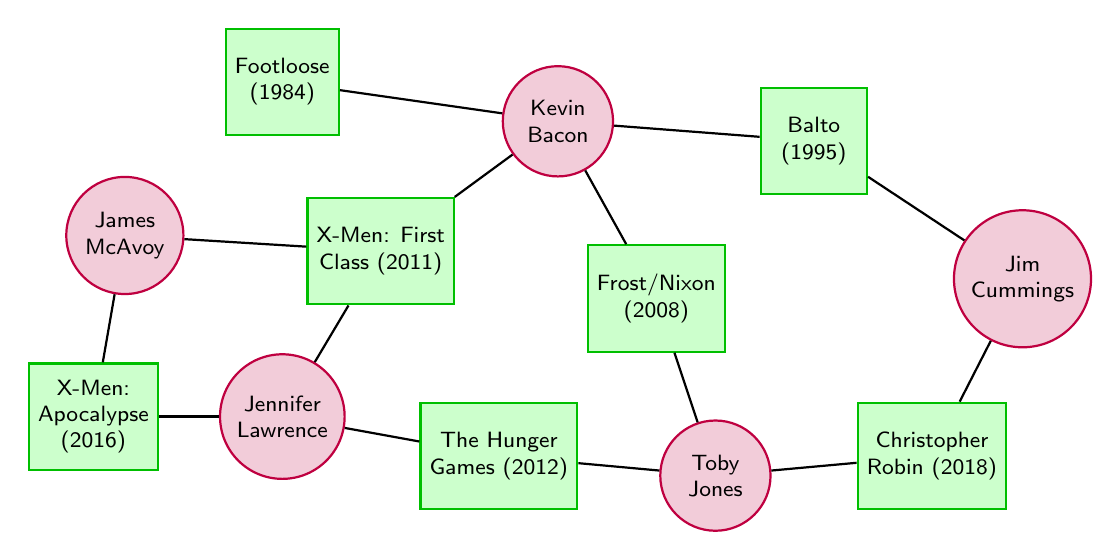
\begin{tikzpicture}
% Set styles for Actor and Movie nodes
\tikzstyle{Actor}=[thick,circle,draw=purple,fill=purple!20!,font=\sffamily\footnotesize,align=center,minimum size=1.4cm]
\tikzstyle{Movie}=[thick,rectangle,draw=green!75!black,fill=green!20!,font=\sffamily\footnotesize,align=center,minimum height=1.35cm,minimum width=1.35cm]
% Nodes
\foreach [count=\i] \x/\y/\t/\n in {
    0/1.25/Kevin\\Bacon/Actor,
    5.9/-.75/Jim\\Cummings/Actor,
    2/-3.25/Toby\\Jones/Actor,
    -3.5/-2.5/Jennifer\\Lawrence/Actor,
    -5.5/-.2/James\\McAvoy/Actor,
    3.25/1/{Balto\\(1995)}/Movie,
    4.75/-3/{Christopher\\Robin (2018)}/Movie,
    1.25/-1/{Frost/Nixon\\(2008)}/Movie,
    .-.75/-3/{The Hunger\\Games (2012)}/Movie,
    -2.25/-.4/{X-Men: First\\Class (2011)}/Movie,
    -5.9/-2.5/{X-Men:\\Apocalypse\\(2016)}/Movie,
    -3.5/1.75/{Footloose\\(1984)}/Movie}
  \node[\n] at (\x,\y) (v\i) {\t};
% Edges
\foreach \i/\j in {1/6, 2/6, 2/7, 3/7, 1/8, 3/8, 3/9,
                   4/9, 1/10, 4/10, 5/10,4/11,5/11,1/12}
  \draw[thick] (v\i) edge (v\j);
\end{tikzpicture}
\caption{A subset of the graph in \texttt{movie\_data.txt}.
Each of these actors have a Bacon number of $1$ because they have all been in a movie with Kevin Bacon.
Every actor in \emph{The Hunger Games} has a Bacon number of at most $2$ because of the paths through Jennifer Lawrence or Toby Jones.}
\label{fig:bfs-network-subset}
\end{figure}

\begin{info} % Note that the movie-actor graph is bipartite.
The movie/actor graph of Problem \ref{prob:bfs-movie-network-init} and Figure \ref{fig:bfs-network-subset} has an interesting property: actors are only directly connected to movies, and movies are only directly connected to actors.
This kind of graph is called \emph{bipartite} because there are two types of nodes, and no node has an edge connecting it to another node of its type.
\end{info}

\begin{warn} % nx.draw() only works on small graphs.
NetworkX \li{Graph} objects can be visualized with \li{nx.draw()} (followed by \li{plt.show()}).
However, this visualization tool is only effective on relatively small graphs.
In fact, graph visualization in general remains a challenging and ongoing area of research.
Because of the size of the dataset, \textbf{do not} attempt to visualize the graph in Problem \ref{prob:bfs-movie-network-init} with \li{nx.draw()}.
\end{warn}

The Six Degrees of Kevin Bacon game poses an interesting question: can any actor be linked to Kevin Bacon, and if so, in how many steps?
The game hypothesizes, ``Yes, within $6$ steps'' (hence the title).
More precisely, let the \emph{Bacon number} of an actor be the number of steps from that actor to Kevin Bacon, only counting actors.
For example, since Samuel L. Jackson was in a film with Frank Whaley, who was in a film with Kevin Bacon, Samuel L. Jackson has a Bacon number of $2$.
Actors who have been in a movie with Kevin Bacon have a Bacon number of $1$, and actors with no path to Kevin Bacon have a Bacon number of $\infty$.
The game asserts that the largest Bacon number is $6$.

NetworkX is equipped with a variety of graph analysis tools, including a few for computing paths between nodes (and, therefore, Bacon numbers).
To compute a shortest path between nodes $u$ and $v$, \li{nx.shortest_path()} starts one BFS from $u$ and another from $v$, switching off between the two searches until they both discover a common node.
This approach is called a \emph{bidirectional BFS} and is typically faster than a regular, one-sided BFS.

\begin{table}[H]
\centering
\begin{tabular}{r|l}
    Function & Description\\
    \hline
    \li{has_path()} & Return \li{True} if there is a path between two specified nodes.\\
    \li{shortest_path()} & Return \textbf{one} shortest path between nodes.\\
    \li{shortest_path_length()} & Return the length of the shortest path between nodes.\\
    \li{all_shortest_paths()} & Yield \textbf{all} shortest paths between nodes. \\
    % \li{average_shortest_path_length()} & Compute the average length of shortest paths from every node to every other node in the graph.
\end{tabular}
\caption{NetworkX functions for path problems. Each accepts a \li{Graph}, then a pair of nodes.}
\end{table}

\begin{lstlisting}
>>> G = nx.Graph({'A': {'B', 'D'},
                  'B': {'A', 'D'},
                  'C': {'D'},
                  'D': {'A', 'B', 'C'}})

# Compute the shortest path between 'A' and 'D'.
>>> nx.has_path(G, 'A', 'C')
<<True>>
>>> nx.shortest_path(G, 'A', 'C')
<<['A', 'D', 'C']>>
>>> nx.shortest_path_length(G, 'A', 'C')
2

# Compute all possible shortest paths between two nodes.
>>> G.add_edge('B', 'C')
>>> list(nx.all_shortest_paths(G, 'A', 'C'))
<<[['A', 'D', 'C'], ['A', 'B', 'C']]>>

# When the second node is omitted from these functions, the shortest paths
# from the given node to EVERY node are computed and returned as a dictionary.
>>> nx.shortest_path(G, 'A')
<<{'A': ['A'], 'D': ['A', 'D'], 'B': ['A', 'B'], 'C': ['A', 'D', 'C']}>>
>>> nx.shortest_path_length(G, 'A')     # Path lengths are defined by the
<<{'A': 0, 'D': 1, 'B': 1, 'C': 2}>>        #  number of edges, not nodes.
\end{lstlisting}

\begin{problem} % Individual shortest paths / Bacon numbers.
Write a method for your class from Problem \ref{prob:bfs-movie-network-init} that accepts two actors' names.
Use NetworkX to compute the shortest path between the actors and the degrees of separation between the two actors (if one of the actors is \li{"Kevin Bacon"}, this is the Bacon number of the other actor).
Note that this number is different than the number of entries in the actual shortest path list, since movies are just intermediate steps between actors.
\label{prob:bfs-actor-path}
\end{problem}

The idea of a Bacon number provides a few ways to analyze the connectivity of the Hollywood network.
For example, the distribution of all Bacon numbers describes how close Kevin Bacon is to actually knowing all of the actors in Hollywood
Someone with a lower average number---for instance, the average \emph{Jackson number}, for Samuel L. Jackson---is, on average, ``more connected with Hollywood'' than Kevin Bacon.
The actor with the lowest average number is sometimes called \emph{the center of the Hollywood universe}.

\begin{problem} % Average Bacon numbers.
\label{prob:bfs-average-bacon-number}
Write a method for your class from Problem \ref{prob:bfs-movie-network-init} that accepts one actor's name.
Calculate the shortest path lengths of every actor in the collection to the specified actor (not including movies).
Use \li{plt.hist()} to plot the distribution of path lengths and return the average path length.
\\(Hint: Use a NetworkX function to compute all path lengths simultaneously; this is significantly faster than calling your method from Problem \ref{prob:bfs-actor-path} repeatedly.
Also, use the keyword argument \li{bins=[i-.5 for i in range(8)]} in \li{plt.hist()} to get the histogram bins to correspond to integers nicely.)
\end{problem}

As an aside, the prolific \href{https://en.wikipedia.org/wiki/Erd%C5%91s_number}{Paul Erd\H{o}s} is the Kevin Bacon equivalent in the mathematical community.
Someone with an \emph{Erd\H{o}s number} of $2$ co-authored a paper with someone who co-authored a paper with Paul Erd\H{o}s.
Having an Erd\H{o}s number of $1$ or $2$ is considered quite an achievement (see \url{https://xkcd.com/599/}).

\newpage

\section*{Additional Material} % ==============================================

\subsection*{Other Hash-based Structures} % -----------------------------------

The standard library has a few specialized alternatives to regular sets and dictionaries.
\begin{itemize}
\item \li{frozenset}: an immutable version of the usual set class.
Frozen sets cannot be altered after creation and therefore lack methods like \li{add()}, \li{pop()}, and \li{remove()}, but they can be placed in other sets and used as dictionary keys.

\item \li{collections.defaultdict}: a dictionary with default values.
For instance, \li{defaultdict(set)} creates a dictionary that automatically uses an empty set as the value whenever a non-present key is used for indexing.
See \href{https://docs.python.org/3/library/collections.html\#defaultdict-examples}{\texttt{https://docs.python.org/3/library/collections.html}} for examples.

\item \li{collections.OrderedDict}: a dictionary that remembers insertion order.
For example, the \li{popitem()} method returns the most recently added key-value pair.
\end{itemize}

\subsection*{Depth-first Search} % --------------------------------------------

A \emph{depth-first search} (DFS) takes the opposite approach of a BFS.
Instead of checking all neighbors of a single node before moving on, it checks the first neighbor, then their first neighbor, then their first neighbor, and so on until reaching a leaf node.
The algorithm then backtracks to the previous node and checks its second neighbor.
While a DFS is rarely useful for finding shortest paths, it is a common strategy for solving recursively structured problems, such as mazes or Sudoku puzzles.

Consider adding a keyword argument to your method from Problem \ref{prob:bfs-traversal} that specifies whether to use a BFS (the default) or a DFS.
To change from a BFS to a DFS, change the visit queue $Q$ to a stack.
You may be able to implement the change in a single line of code.

\subsection*{The Center of the Hollywood Universe} % --------------------------

Computing the center of the universe in a graph amounts to solving Problem \ref{prob:bfs-average-bacon-number} for every node in the graph.
This is computationally expensive, but since each average number is independent of the others, the problem is a good candidate for \emph{parallel programming}, which divides the computational workload between multiple processes.
Even with parallelism, however, computing the center of the Hollywood universe may require significant computational time and resources.

\subsection*{Shortest Paths on Weighted Graphs} % -----------------------------

The graphs presented in this lab are \emph{unweighted}, meaning all edges have the same importance.
A \emph{weighted graph} assigns a weight to each edge, which can usually be thought of as the distance between the two adjacent nodes.
The shortest path problem becomes much more complicated on weighted graphs, and requires additions to the plain BFS.
The standard approach is \emph{Dijkstra's algorithm}, which is implemented as \li{nx.dijkstra_path()}.
Another approach, the \emph{Bellman-Ford algorithm}, is implemented as \li{nx.bellman_ford_path()}.
